\chapter{Kompontentendesign}
\label{chap:komponentendesign}


%%% IN diesem Kapitel werden für die einzelnen services der Tech stack geklärt etc.!!!

\begin{figure}
    \label{figure:diagrammanordnungsverfahren}
    \begin{center}
    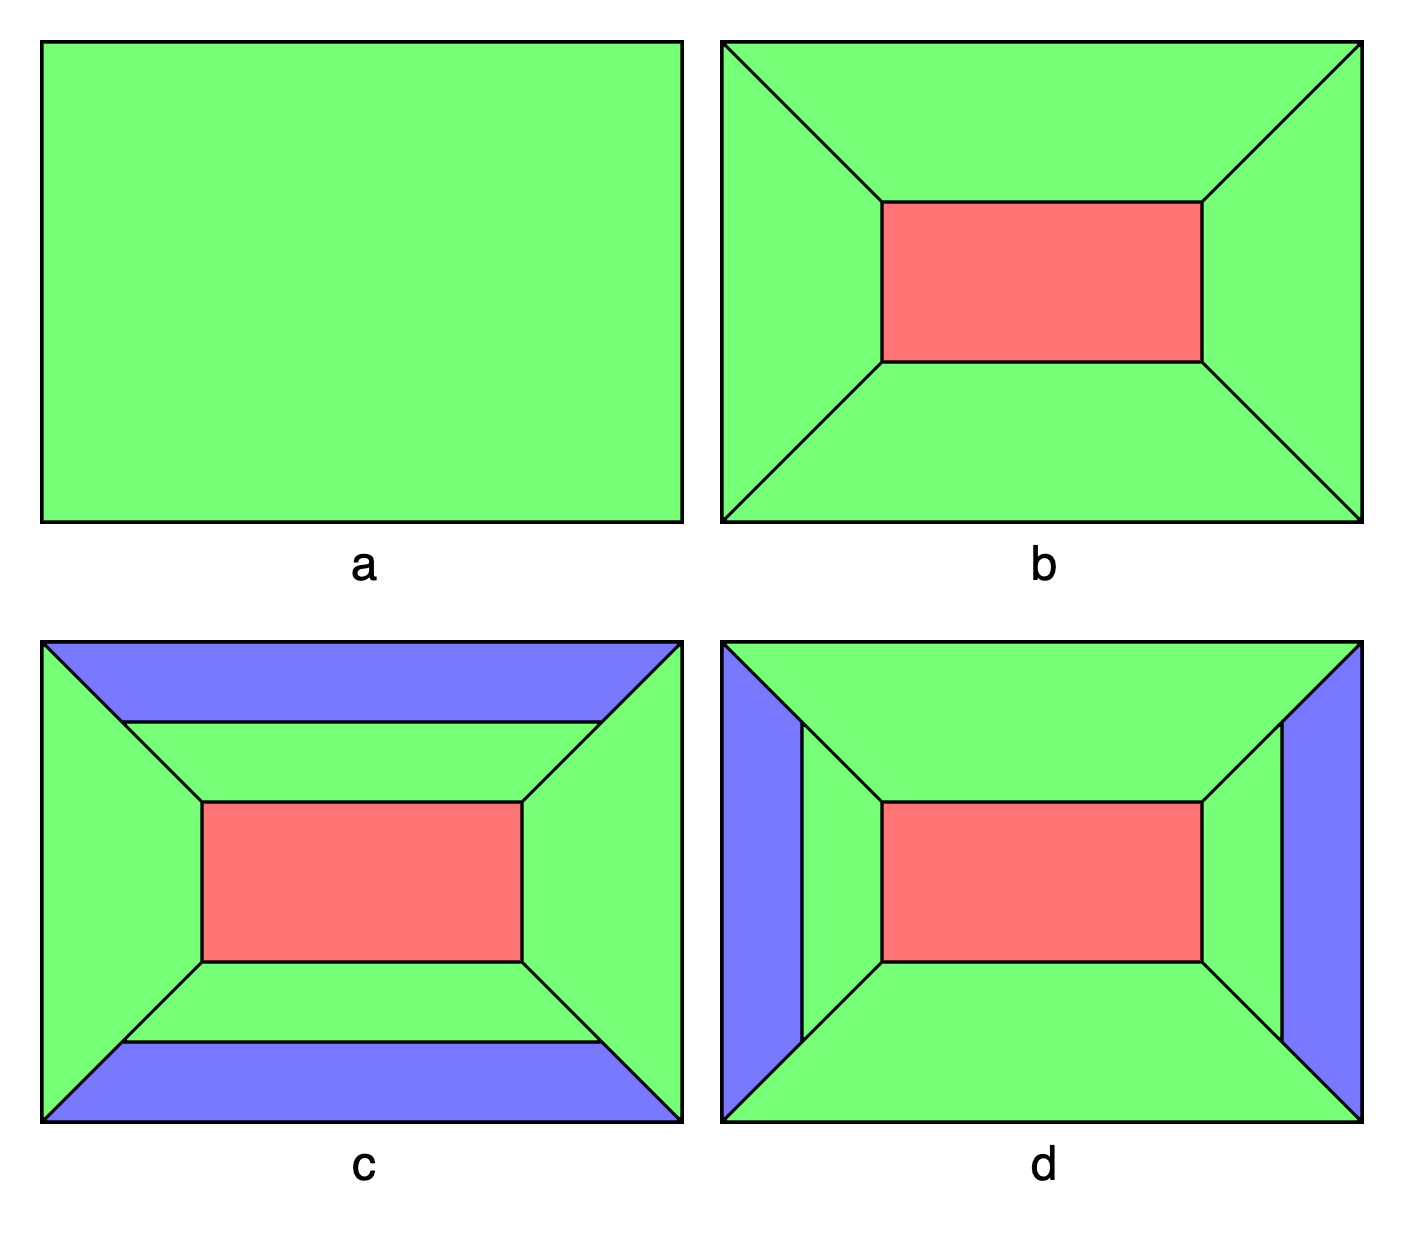
\includegraphics[scale=0.2]{img/abbildungen/Diagrammanordnunsverfahren}
    \end{center}
    \caption{Diagrammanordnunsverfahren}
\end{figure}

\section{Resource Management API}
\label{sec:resourcemanagementapi}

\section{Data Delivery API}
\label{sec:datadeliveryapi}

\section{Protokolle}
\label{sec:protokolle}
% Also question ? Send batches which server can immediately handle
% or does the server has to wait till all the data has arrived
\subsection{HTTP 2}
\label{subsec:http2}

\subsection{Websockets}
\label{subsec:websockets}

% Cite this text: Another useful feature of being able to establish a connection using
% HTTP is the ability to use HTTP authentication semantics for the socket,
% such as the Authorization header for Basic Auth or Bearer Token Auth.
% https://codeburst.io/why-you-don-t-need-socket-io-6848f1c871cd

\section{Schnittstellengestaltung}
\label{sec:schnittstellengestaltung}

\subsection{Open API 3.0}
\label{subsec:openapi3}

\subsection{AsyncAPI}
\label{subsec:asyncapi}

\subsection{GraphQL Subscriptions}
\label{subsec:graphqlsubscriptions}

\section{Sicherheit}
\label{sec:sicherheit}

\subsection{Middlewares}
\label{subsec:middlewares}

\subsection{JWT}
\label{subsec:jwt}
% JWT vs Session
% Whitelist statt Blacklist

\section{Skalierbarkeit}
\label{sec:skalierbarkeit}
